\begin{question}
\noindent Triangle $T$ has vertices $A$, $B$ and $C$, shown on the grid below.

\begin{center}
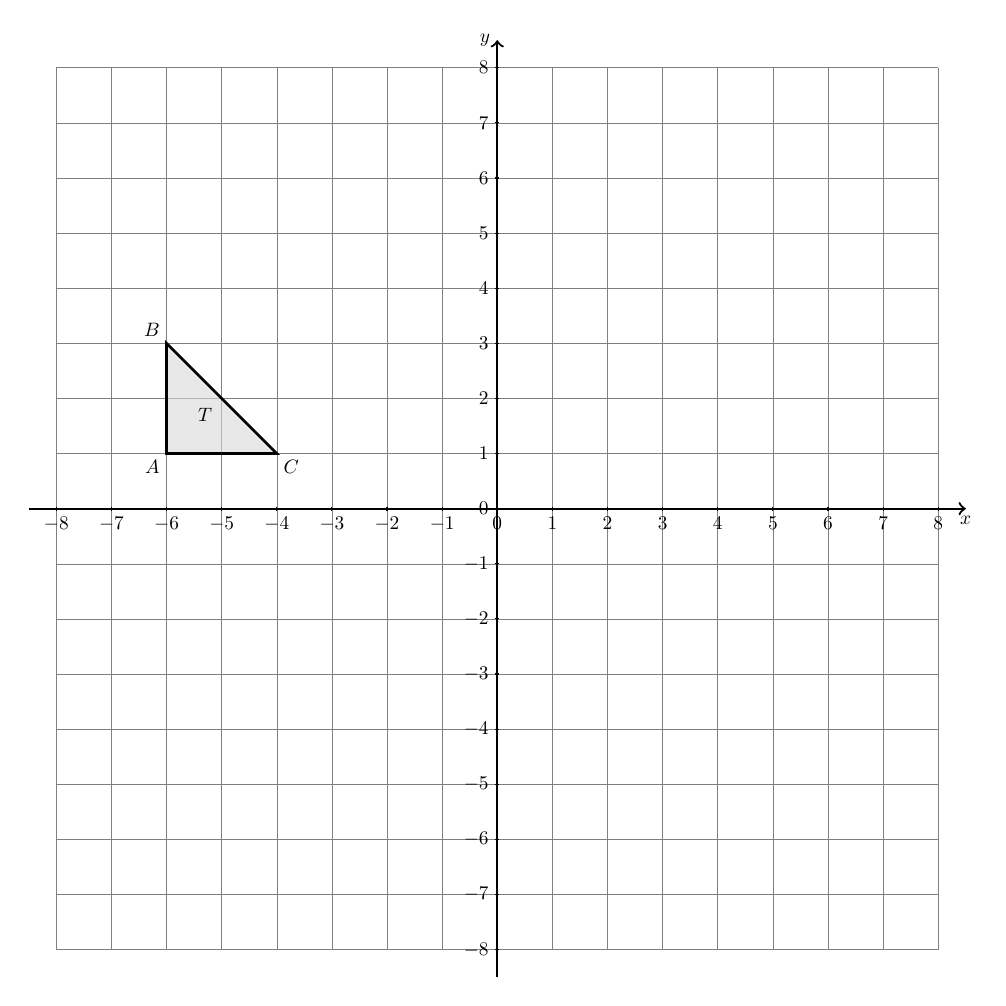
\begin{tikzpicture}[scale=0.7, transform shape]
    \definecolor{borderColour}{HTML}{000000}
    \definecolor{fillColour}{HTML}{D8D8D8}

    \def\axisLimit{8}

    \draw[step=1cm,gray,very thin] (-\axisLimit,-\axisLimit) grid (\axisLimit,\axisLimit);

    \draw[thick,->] (-\axisLimit-0.5,0) -- (\axisLimit+0.5,0) node[anchor=north] {$x$};
    \draw[thick,->] (0,-\axisLimit-0.5) -- (0,\axisLimit+0.5) node[anchor=east] {$y$};

    \foreach \x in {-\axisLimit,...,\axisLimit}
        \draw (\x cm,1pt) -- (\x cm,-1pt) node[anchor=north] {$\x$};
    \foreach \y in {-\axisLimit,...,\axisLimit}
        \draw (1pt,\y cm) -- (-1pt,\y cm) node[anchor=east] {$\y$};

    \coordinate (A) at (-6,1);
    \coordinate (B) at (-6,3);
    \coordinate (C) at (-4,1);

    \filldraw[fill=fillColour, draw=borderColour, line width=1pt, fill opacity=0.6] (A) -- (B) -- (C) -- cycle;

    \node[below left] at (A) {$A$};
    \node[above left] at (B) {$B$};
    \node[below right] at (C) {$C$};
    \node at (-5.3,1.7) {$T$};

\end{tikzpicture}
\end{center}

\noindent Triangle $T$ is translated by the vector $\begin{pmatrix} 7 \\ -5 \end{pmatrix}$ to give triangle $T_1$.

\noindent Triangle $T_1$ is then reflected in the line $y = 1$ to give triangle $T_2$.

\begin{enumerate}
    \item[(a)] Find the coordinates of the vertices of triangle $T_1$.

    \vspace{4cm}
    \answerplain{2}

    \item[(b)] Find the coordinates of the vertices of triangle $T_2$.

    \vspace{4cm}
    \answerplain{2}
\end{enumerate}
\end{question}
